\section{Design}

The results of the prestudy allows us to justify the design of a platform for granularly targeting adverts and providing interaction within adverts. This section will cover the design of this platform, as well as how this platform can be demonstrated within a personalised TV channel -- a TV channel tailored towards viewers specifically on which programmes and adverts are recommended based on information about the viewer. Our implementation (Section~\ref{sec:implementation}) of this personal TV channel is called \textit{Your4.tv}.

We'll start by discussing how adverts will be targeted through \textit{campaigns} -- a set of restrictions on viewers that adverts must conform to in order to be shown. Following this, we'll devise a method to allow interactivity in adverts. We also describe how we can collect statistics that this platform would offer about advert usage. In order to demonstrate the usage of these adverts, we then discuss the design of \textit{Your4.tv}, a personalised TV channel, which will utilize a recommender system to select programmes that the viewer will want to watch.

\subsection{Overview}

	Due to the large number of topics this platform encompasses, it was important that we understood what tasks would be involved. Figure~\ref{fig:designing} shows an early plan, demonstrating the major parts and types of information that would be required. This overview shows that a personalised TV stream would have programmes selected by a recommender, which learns from a user's preference. Targeted interactive adverts be selected based on information about the user and their context.

	The diagram categorises the tasks involved into client-side development (blue), statistics (yellow), recommendation (red), streaming (green) and overlays (black). This allows these tasks to be allocated to team members effectively.

	\begin{landscape}
	\begin{figure}[th]
		\centering
		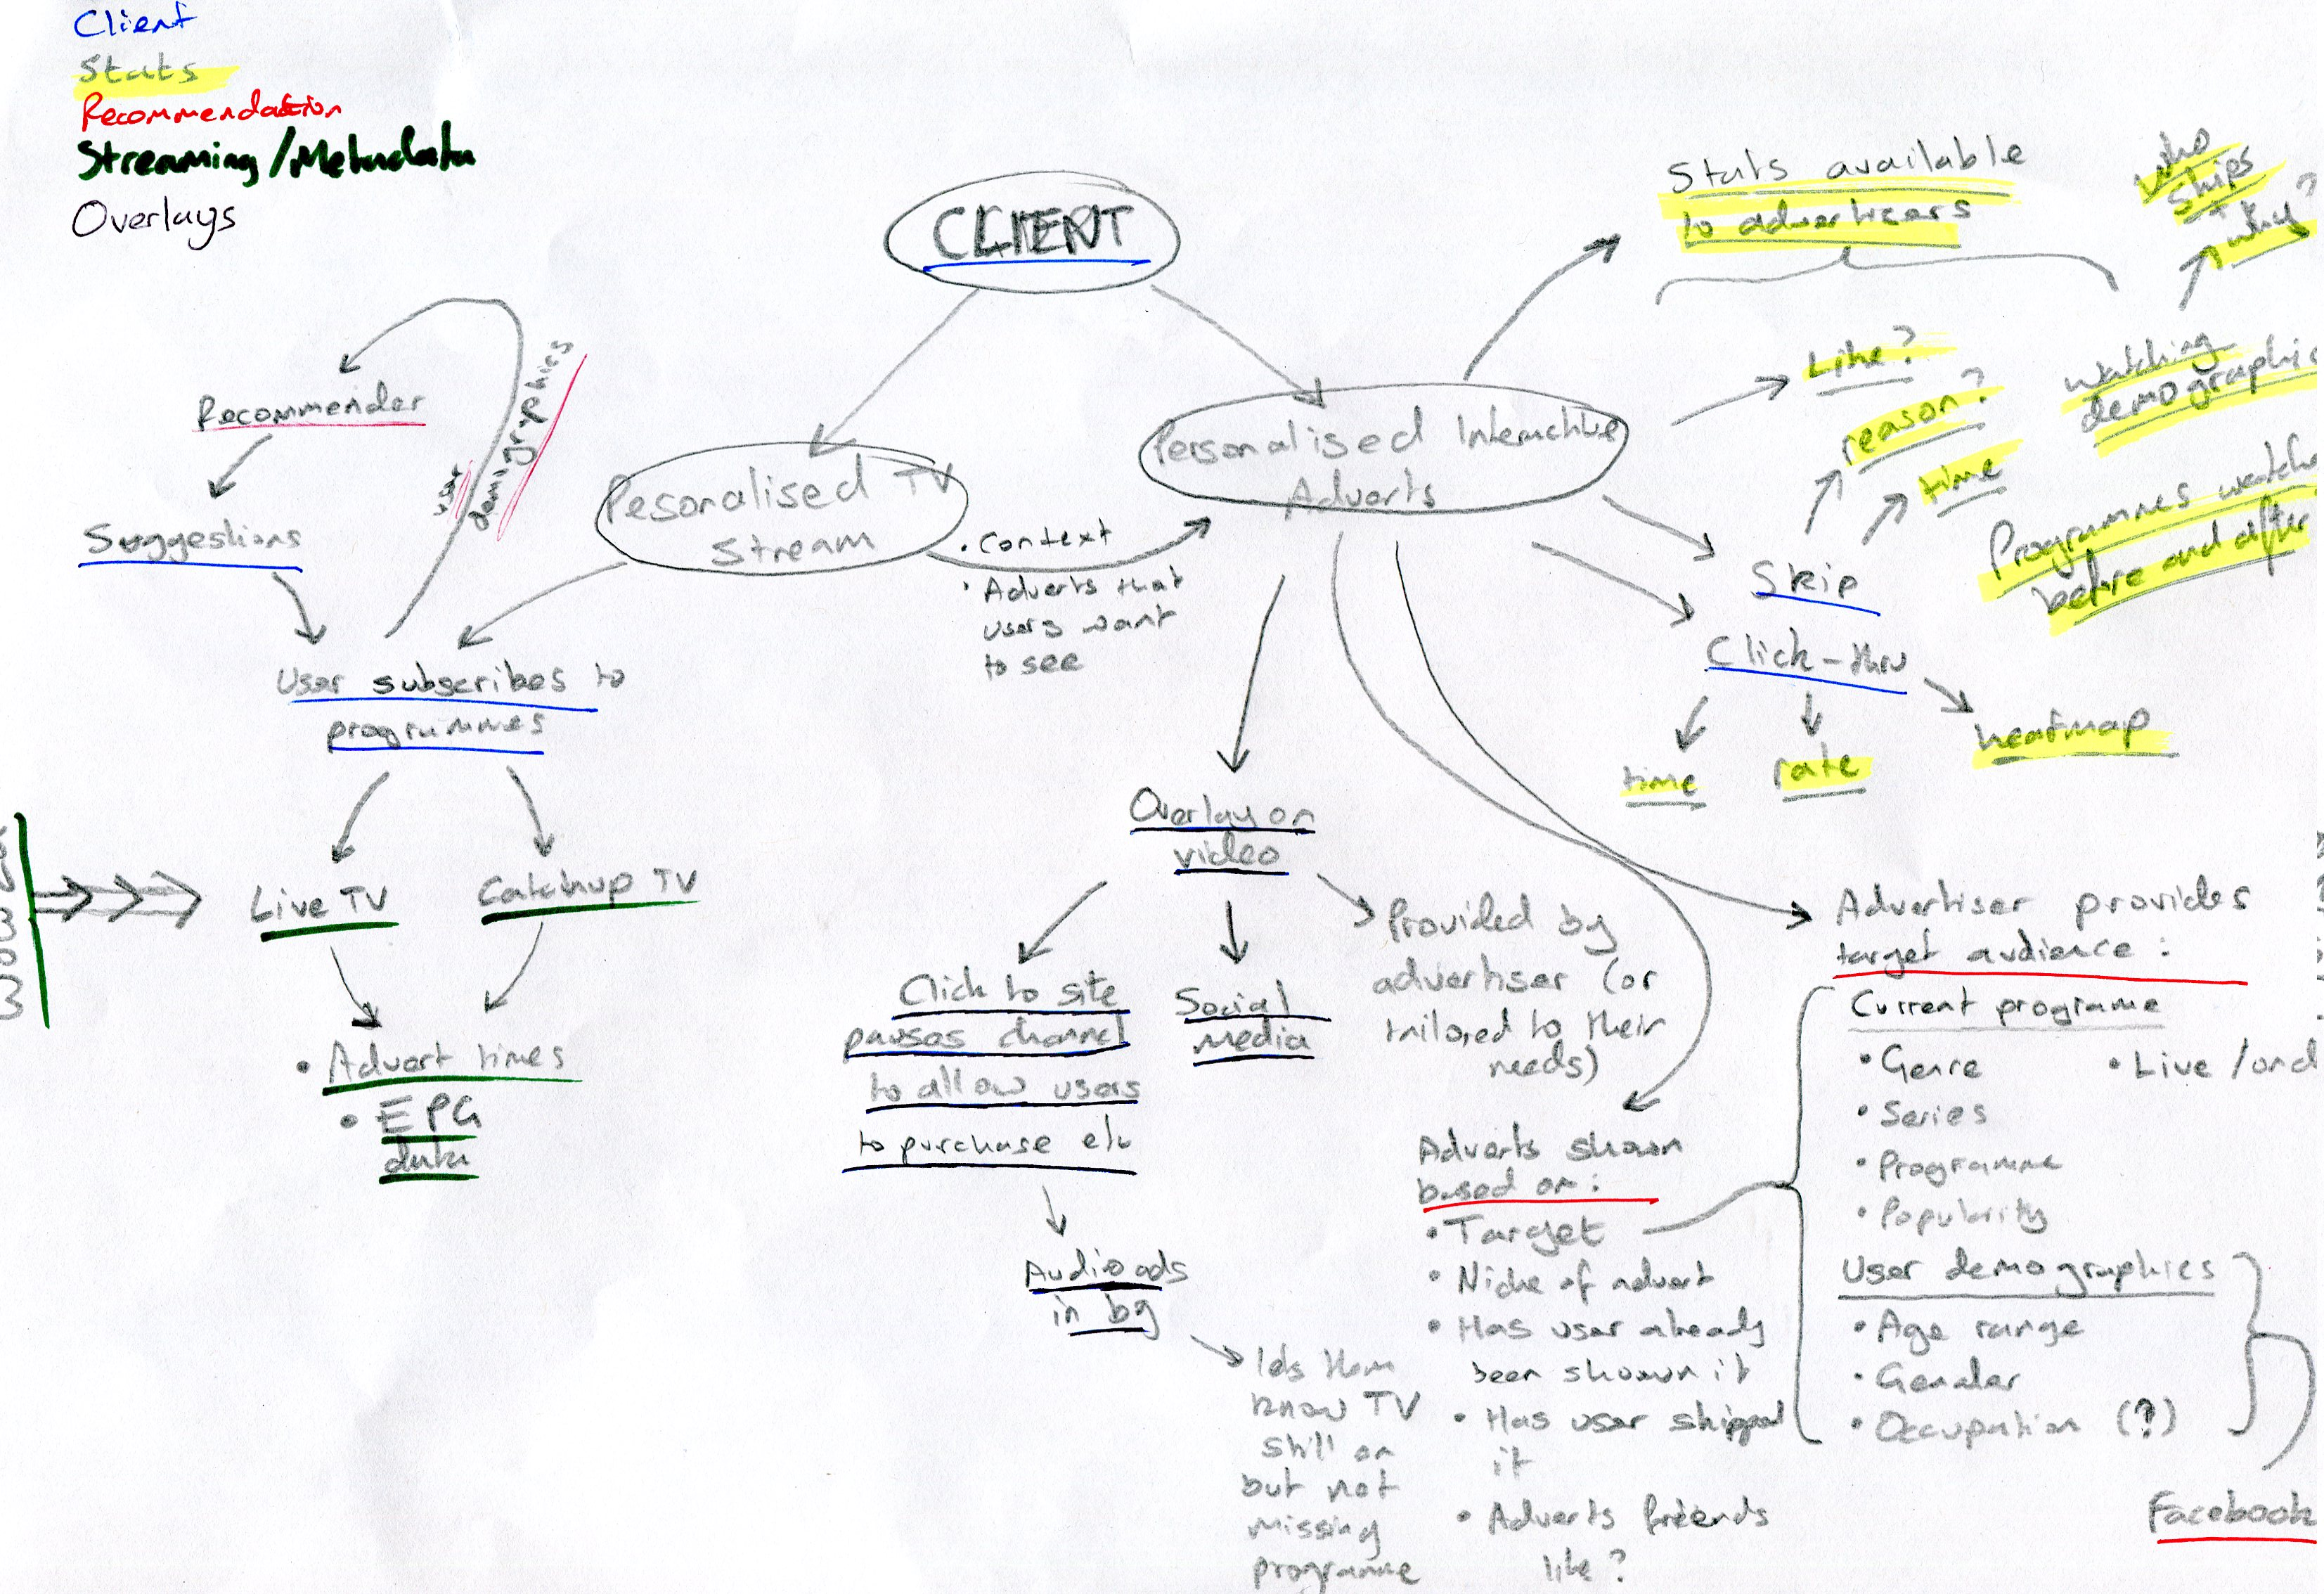
\includegraphics[height=\textwidth]{images/design.jpg}
		\caption{Design stage planning}
		\label{fig:designing}
	\end{figure}
	\end{landscape}
	\newpage

\subsection{Targeting adverts}
	\label{sec:design_adverts}

	Advert relevance is known to increase user engagement \citep{nettelhorst2012effects, advertising_engagement} and enjoyment \citep{yahoo-intrusive-advertising}, positively influencing the user experience. Furthermore, our prestudy (Section~\ref{sec:prestudy}) revealed that, out of all the criteria given, advert relevance had the greatest influence on the likelihood of an advert being watched. The use of granular targeting would allow advertisers to specify very specific target markets based on demographics, browsing habits and contextual information. 
	%% This is tautologically true
	% As shown in [cite], adverts targeted specifically towards individuals are, in general, more relevant to that individuals personal interests.

	The usage of internet-connected devices allows the capturing of information about a user, allowing this granular targeting. In the design of our advertising platform, we take the notion of an advert campaign, 
	%% Who wrote this? Put your citations in!
	%as used by [cite] in [some system], 
	and allow an advert to be targeted towards people based on personal information (such as age, gender and occupation), usage data (such as viewing history) and contextual information (such as time of day and what programme they are watching).

	In the context of live TV, these targeted adverts would replace adverts that are streamed as part of the channel by the broadcaster. This advert replacement has been implemented successfully previously as part of Project4, as described in Section~\ref{sec:motivation_inqb8r}. In addition, these advert breaks could be placed in between non-live streamed programmes.

	\subsubsection{Skipping adverts}

	%% Has anybody actually got a paper on this?
	% [cite] discusses the use of skip functionality in adverts in [system]. 
	Users were able to skip adverts that they did not enjoy, such that they would be presented with a different advert for the remainder of the advert break.
	%% Where did this statistic come from?
	% x\% of users were satisfied that by skipping adverts, they would be more likely to be presented with adverts that were of interest to them.
	Furthermore, our prestudy revealed that 64\% of individuals felt that skip functionality would influence the attention they would pay to adverts.

	From this, we wish to include skip functionality as part of our design: a user may skip an advert in order to be presented with a different advert, and may do so until the advert break has finished. In order to expand on this, we will ask users why they chose to skip an advert, presenting options much like Facebook advert skip options as discussed in 
	% This reference is broken
	Section~\ref{subsection:backgroundStats}. This will allow advertisers to collect information on why individuals skip adverts and allow users to effectively block adverts from being shown again.

	\subsubsection{Advert campaigns}

	Any advert may be targeted towards individuals by assigning that advert to a campaign; an advert may be in as many campaigns as the advertiser needs, and a campaign may include any number of adverts. A campaign is given a set of restrictions, where the adverts belonging to a particular campaign are shown whenever the campaign restrictions are met. Restrictions may apply to programmes, users and times, where the attributes that can be restricted are:

	\begin{center}
		\begin{tabular}{c c r l}
			\toprule
			\textbf{Programmes} & \textbf{Times} & \multicolumn{2}{c}{\textbf{Users}} \\
			\midrule
			genre & time of day & ~~gender & latitude \\ % The two non-breaking spaces are so the table looke a little nicer. ( Nice olde English there ). Whye, how kinde of you goode sir.
			individual programme & weekday & age & longitude \\
			liveness & & &  occupation \\
			\bottomrule
		\end{tabular}
	\end{center}

	Attributes may have multiple restrictions, where the restrictions are discrete points or continuous ranges where appropriate (e.g., ages restrictions are specified as ranges, and genre restrictions as points). When a campaign has multiple restrictions on a single attribute, that attribute is considered satisfied if any of its restrictions are satisfied; e.g.: if a campaign has weekday restrictions of Monday and Wednesday, the weekday restriction is considered satisfied on either a Monday or a Wednesday. A campaign only applies when all of its restrictions are satisfied, though a campaign need not have restrictions for all of the above attributes, or indeed any restrictions at all.

	Whenever a campaign is satisfied, its adverts are shown with a frequency directly proportional to the value of a campaign metric that we call \textit{nicheness}. We define nicheness, $n$, as:
	$$
		n = \frac{(1-n_\text{programme}) + (1-n_\text{time}) + (1-n_\text{user})}{3}
	$$
	where
	\begin{align*}
		n_\text{programme} &= 1 - \frac{\text{satisfying programmes}}{\text{total programmes}} \\
		n_\text{time} &= 1 - \frac{\text{satisfied time during campaign}}{\text{total time during campaign}} \\
		n_\text{user} &= 1 - \frac{\text{satisfying users}}{\text{total users}}
	\end{align*}

	In other words, for a particular person, programme and time in which multiple campaigns apply, campaigns with a higher nicheness will have their adverts displayed more often. This design decision was made to reward advertisers for creating niche campaigns over broad campaigns. By encouraging a greater number of more highly targeted advertisements in this way, users will be shown a far more relevant advert set. Given a set of satisfied campaigns $\mathbb{C}$ where each campaign is a set of adverts, the probability that an advert $a$ is shown from a particular campaign is:
	$$
		P(a|\mathbb{C}) =
		\frac{
			\displaystyle \sum_{c \in \mathbb{C}}
			\begin{cases}
				\frac{n_c}{\left|c\right|}, & a \in c \\
				0, & \text{otherwise}
			\end{cases}
		}{
			\displaystyle \sum_{d \in \mathbb{C}} n_d
		}
	$$
Which stems from the algorithm: A campaign is picked from $\mathbb{C}$ with a probability equal to its nicheness in proportion to the sum of nichenesses in $\mathbb{C}$; from this campaign, an advert is picked with equal probability from all the adverts that apply to the campaign. While the above equation becomes singular if every campaign in $\mathbb{C}$ has a nicheness of 0, the algorithm implemented allows this; this is the only case when a campaign with nicheness 0 can ever be returned, in which case a campaign is chosen with equal probability. This is desirable, as campaigns with no restrictions on them may be created, showing adverts to users to whom no targetted adverts apply.

\subsection{Advertiser statistics}

	As discussing in Section~\ref{sec:background_stats}, TV devices which transmit usage data account for less than 0.5\% of TV viewers within the USA, representing a very small sample of TV viewers. However, internet analytics services, such as YouTube and Google Analytics, allow fine-granular statistics to be collected about users of web-based services, including what material individuals view, how long for and even an individuals location when they accessed the material. Such information would be extremely valuable to advertisers.
	%% WHO??
	%, with [cite] demonstrating a demand for newer, higher-granular statistics.

	Using an internet-enabled device allows two way communication -- a device may receive video from a streaming service to present to the user and send information about the user back to the streaming service. We can incorporate this as part of our design, which would allow us to collect three types of information:
	\begin{description}
	\item[Demographic information] age, gender and occupation;
	\item[Contextual information] time of day, location and what programme the viewer is watching;
	\item[Usage information] what programmes and adverts the viewer has watched in the past, when and where users have clicked on adverts.
	\end{description}

	The usage information would allow advertisers to fine-tune adverts and campaigns towards their target demographic, focusing on who watches the advert and how they they are interacted with. Furthermore, with the skip functionality, advertisers could establish when users are most likely to skip during an advert and why.

\subsection{Personalised TV channel}

	The proposed information used for advert targeting, as described in Section~\ref{sec:design_adverts}, includes contextual information, such as what programme a user is watching, and a viewers usage history, such as programmes they've watched in the past. In order to provide this information, we wish to use the advert platform on top of a TV streaming services. We devised a personalised TV streaming services for this purpose, which would ensure that a user is watching TV programmes that they are interested in them. If programmes that are shown to a user are of interest to them, then adverts shown to them should cater more to their interest.

	At the centre of this personalised TV channel is a recommender system which learns from a user's preferences towards particular programmes and subsequently recommends programmes based on their interests. The programmes that would be available to this recommender system would be any programmes that have been streamed on Channel~4 (or it's sister channels -- see Section~\ref{backgroundChannel4}).

	\subsubsection{Programme recommendation}

		A user who accesses this system would be presented with a TV channel populated with a list of programmes as recommended by a programme recommendation system.  This system recommends programmes specifically, and is separate from the targeted advert retriever (described in Section~\ref{sec:design_adverts}).

		At an abstract level, each programme is given a vector $\mathbf{p}$, which describes what the programme is like. The programme vector $\mathbf{p}$ lies within the programme space $\mathcal{P}$, and is calculated from a vector of programme information $\mathbf{i}$ using the function $v_p$ ($\mathbf{p} = v_p(\mathbf{i})$). The concrete implementation of this used in \textit{Your4.tv} is that $\mathcal{P}$ is 19-dimensional, where each dimension represents one of the genres:

		\begin{center}
			\emph{\footnotesize{
				\begin{tabular}{c c c c c}
					Action and Adventure & Animation & Children & Comedy & Documentary \\
					Drama & Game Show & Home and Garden & Mini-Series & News \\
					Reality & Science-Fiction & Fantasy & Soap & Special Interest \\
					Sport & Talk Show & Western & Unclassified &
				\end{tabular}
			}}
		\end{center}


		This is the full set of allowable genres on The Tvdb\footnote{TheTVDB -- \footurl{http://thetvdb.com}} plus `Unclassified', which is reserved for programmes which $v_p$ cannot assign an appropriate vector. To map a programme into this space, $v_p$ uses the supplied programme name to query the Tvdb API\footnote{TheTVDB Programmers API -- \footurl{http://thetvdb.com/wiki/index.php/Programmers\_API}} for a programme's genres, and returns a binary vector of genre memberships (for each element: 1 if the programme belongs in genre; 0 otherwise). As an example, the programme `Grand Designs' has genres \emph{Documentary}, \emph{Home and Garden} and \emph{Reality}, so would be assigned the vector:
		$$
		\left[0,0,0,0,1,0,0,1,0,0,1,0,0,0,0,0,0,0,0\right]^T
		$$

		So that a user may be recommended programmes, each user is given a vector, $\mathbf{u}$, also within the space $\mathcal{P}$, which represents the user's ideal programme. This user vector is initialised with the function $v_u$, which takes a vector of a user's demographic information, $\mathbf{d}$, and returns the user vector, $\mathbf{u}$ ($\mathbf{u} = v_u(\mathbf{d})$). The actual demographics in $\mathbf{d}$ are constrained by the target audience, the training data available and the user data available, and as a result only gender is considered ($\mathbf{d} \in \left\{{ \left[ 0\right] ,\left[ 1\right] }\right\} $). The function $v_u$ is learned using a set of training data containing mappings between users, their demographics and shows they enjoy.

		While a user uses \textit{Your4.tv}, their actions influence their user vector. Upon giving a programme a rating, $\mathbf{u}$ is moved either towards or away from $\mathbf{p}$ by an amount which depends upon the magnitude of the rating, the initial distance between $\mathbf{u}$ and $\mathbf{p}$, and the learning rate of the recommender which may be tweaked or made inversely proportional to the number of ratings made by the user. While an adaptive learning rate will result in a simulated-annealing type search in the programme space, a constant learning rate will continue adapting recommendations to the user's current mood, which should not be assumed to be static. The exact change to $\mathbf{u}$, where $\mathbf{u}_{i}$ is the $i^{th}$ component of vector $\mathbf{u}$, $\mathbf{u}'$ is the new user vector, $0 \leq L \leq 1$ is the learning rate and $-1 \leq r \leq 1$ is the rating given is given by:
		% Can use dcases in mathtools to make the fractions in the conditional more readable (bigger).
		$$
			\mathbf{u}_{i}' =
			\mathbf{u}_{i} + \begin{cases}
				\left|\mathbf{q}_i\right|Lr \times \frac{\mathbf{q}_i}{\left|\mathbf{q}_i\right|},&
					\text{if } r\geq 0\\
				(1-\left|\mathbf{q}_i\right|)Lr \times \frac{\mathbf{q}_i}{\left|\mathbf{q}_i\right|},&
					\text{otherwise}
			\end{cases}
		$$
		where $q$ is the abbreviated difference between the programme and user vector:
		$$
			\mathbf{q} = \mathbf{p}-\mathbf{u}
		$$
		Because of division by 0 for the case when the user and programme vectors are, on a particular dimension, identical ($\mathbf{q}=0$), a special case was required:
		$$
			\mathbf{u}_{i}' =
			\mathbf{u}_{i} + \begin{cases}
				0,&
					\text{if } r\geq 0\\
				\operatorname{sign}(\operatorname{random}()-0.5)\times Lr,&
					\text{otherwise}
			\end{cases}
		$$

		Genres from Tvdb were chosen as a basis for $\mathcal{P}$, as this solved the problem of finding training data for the learned function $v_u$. The MovieLens 1M dataset\footnote{\url{http://www.grouplens.org/node/73}} was downloaded, and the movies mapped to their corresponding Tvdb genres, giving a large dataset of user demographics, movie ratings, and movie vectors within the programme space $\mathcal{P}$ which serve as suitable training data. To map new programmes into the $\mathcal{P}$, $v_p$ looks up the Tvdb genres for a given programme, using these to construct $\mathbf{p}$.

			\begin{figure}[h!]
				\begin{center}
				\begin{subfigure}[t]{0.32\textwidth}
					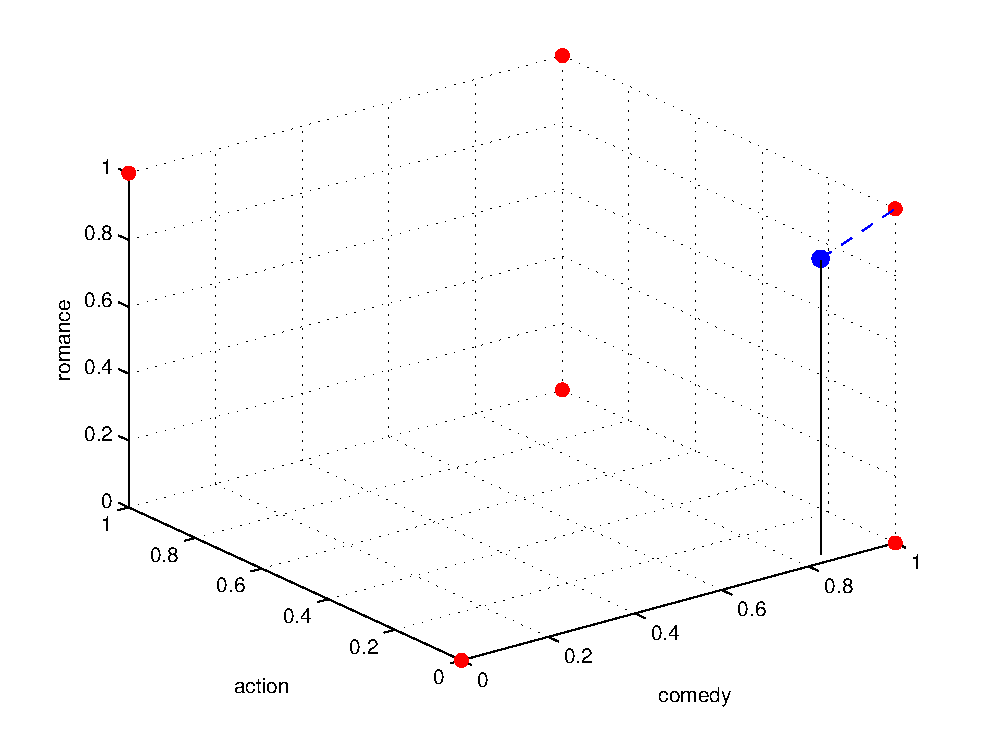
\includegraphics[width=\textwidth]{images/recommender_1.pdf}
					\caption{A user is recommended the programme which minimises $||\mathbf{p} - \mathbf{u}||$.}
				\end{subfigure}
				\begin{subfigure}[t]{0.32\textwidth}
					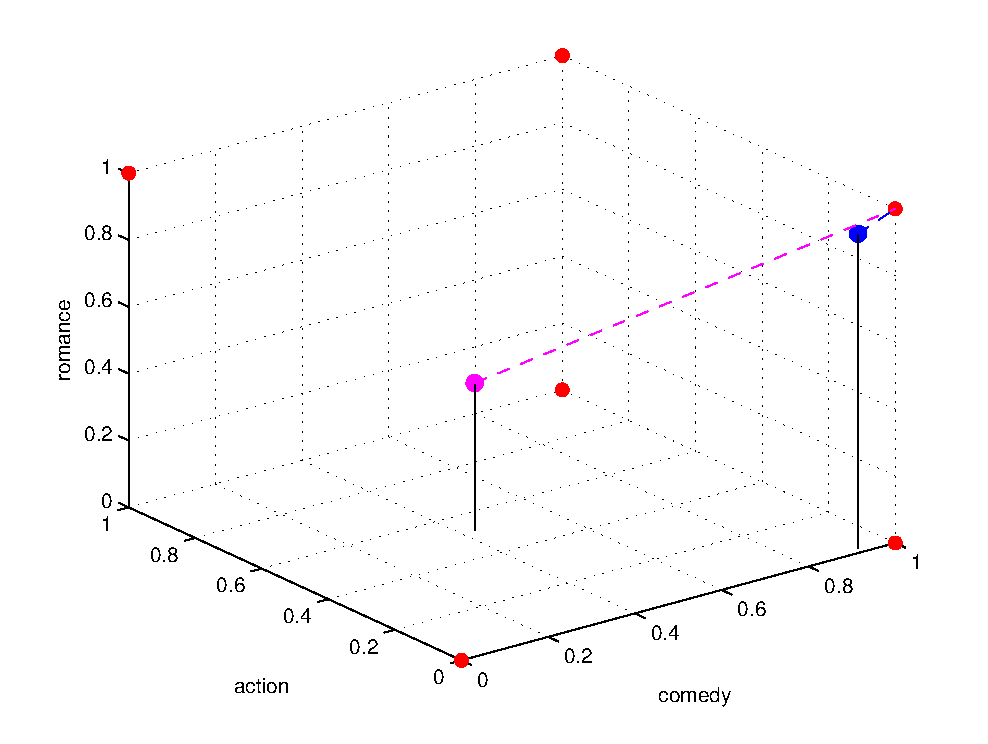
\includegraphics[width=\textwidth]{images/recommender_2.pdf}
					\caption{Giving a rating modifies $\mathbf{p}$. Here, a positive rating results in the blue (righthand) and a negative rating gives the purple (lefthand) pin.}
				\end{subfigure}
				\begin{subfigure}[t]{0.32\textwidth}
					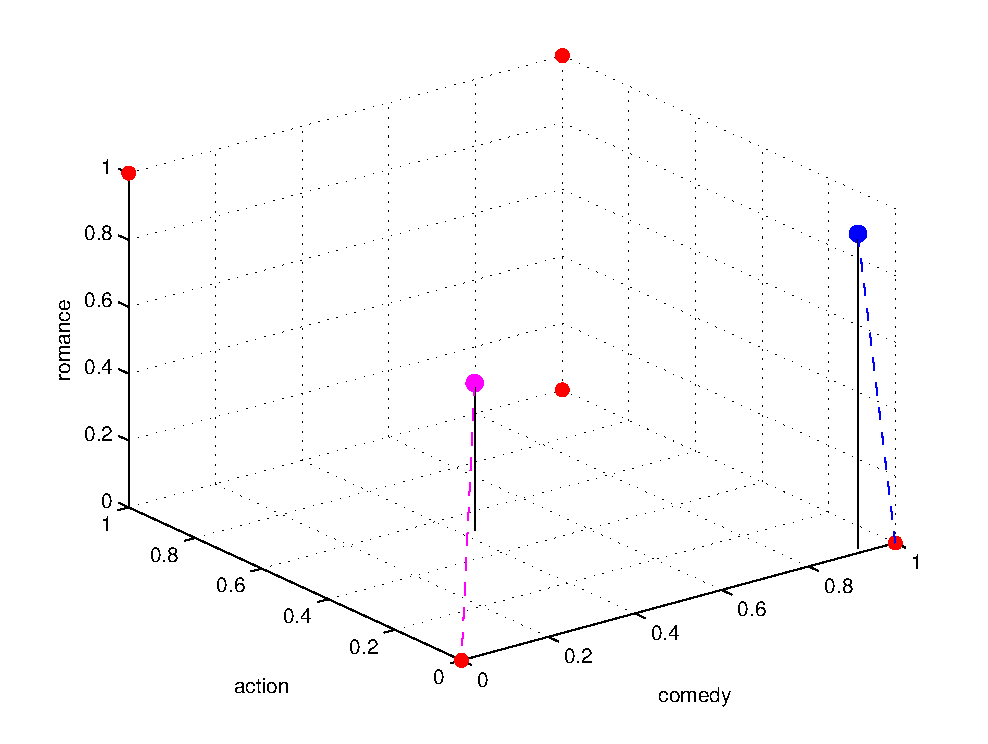
\includegraphics[width=\textwidth]{images/recommender_3.pdf}
					\caption{The programme just watched/skipped is removed from the users programme pool, and the user is recommended a new different programme.}
				\end{subfigure}
				\caption{Visualisation of how the state of an example 3-dimensional version or the recommender described above changes during use. The axes used in this example are romance, action and comedy; a subset of the 18 dimensions in the actual implementation.}
				\label{fig:recommender_example}
			\end{center}
		\end{figure}

		The space $\mathcal{P}$ is, by design, coupled only with the functions $v_u$ and $v_p$. As a result of this, $v_p$ may be modified, changing the structure of $\mathcal{P}$, as long as $v_u$ is re-learnt using the new programme representation. This is desirable, as programme representations better suited to recommendation are possible; i.e., more similar programmes are closer together, more different programmes are further apart, and similar programmes are not given identical representations. Possible ways of accomplishing this are discussed in section~\ref{sec:further_work_recommender}.

	\subsubsection{Programme availability}

		The programmes available would be any show that has been broadcast on Channel~4 (or it's sister channels) that we record. Due to storage constraints, we restrict the time which we keep programmes to 7 days - so any programme that has broadcast on these channels in the past 7 days will be available for the programme recommender to recommend.
